% Template for PLoS
% Version 1.0 January 2009
%
% To compile to pdf, run:
% latex plos.template
% bibtex plos.template
% latex plos.template
% latex plos.template
% dvipdf plos.template

\documentclass[10pt]{article}

% amsmath package, useful for mathematical formulas
\usepackage{amsmath}
% amssymb package, useful for mathematical symbols
\usepackage{amssymb}

% graphicx package, useful for including eps and pdf graphics
% include graphics with the command \includegraphics
\usepackage{graphicx}

% cite package, to clean up citations in the main text. Do not remove.
\usepackage{cite}

\usepackage{color} 

% Use doublespacing - comment out for single spacing
\usepackage{setspace} 
\doublespacing

\usepackage{multirow}

% Text layout
\topmargin 0.0cm
\oddsidemargin 0.5cm
\evensidemargin 0.5cm
\textwidth 16cm 
\textheight 21cm

% Bold the 'Figure #' in the caption and separate it with a period
% Captions will be left justified
\usepackage[labelfont=bf,labelsep=period,justification=raggedright]{caption}

% Use the PLoS provided bibtex style
\bibliographystyle{plos2009}

% Remove brackets from numbering in List of References
\makeatletter
\renewcommand{\@biblabel}[1]{\quad#1.}
\makeatother


% Leave date blank
\date{}

\pagestyle{myheadings}
%% ** EDIT HERE **


%% ** EDIT HERE **
%% PLEASE INCLUDE ALL MACROS BELOW

%% END MACROS SECTION

\begin{document}

% Title must be 150 characters or less
\begin{flushleft}
{\Large
\textbf{RNA-Seq Assembly Discovers Many Splice Variants}
}
% Insert Author names, affiliations and corresponding author email.
\\
Likit Preeyanon$^{1}$, 
Jerry B. Dodgson$^{1}$
Hans Cheng$^{2}$, 
C. Titus Brown$^{3,1 \ast}$
\\
\bf{1} Microbiology and Molecular Genetics, Michigan State University, East Lansing, MI, USA.
\\
\bf{2} Avian Disease and Oncology Laboratory, East Lansing, MI, USA.
\\

\bf{3} Department of Computer Science and Engineering, Michigan State University, East Lansing, MI, USA.
\\
$\ast$ E-mail: ctb@msu.edu
\end{flushleft}

% Please keep the abstract between 250 and 300 words
\section*{Abstract}
Splice variants play an important role in biological systems, especially in the
immune system and the central nervous system. An expression profile of splice
variants has been shown to be a better signature of some diseases than an
overall gene expression profile~\cite{zhang2013isoform}. However, for most
organisms, available gene models such as Ensembl may not include all splice
variants expressed in RNA-Seq data. Reference-guided (e.g.
Cufflinks~\cite{Trapnell:2010kd}) and de novo assembly (e.g.
Velvet/Oases~\cite{Schulz:2012je}) methods are available for building gene
models from RNA-Seq reads. However, we found that both types of method recovered
distinct sets of splice variants.  In this article, we introduce a pipeline that
can combine transcripts from {\em de novo} assembly and other gene models to
constructs gene models that include more splice variants. We also described a
method called local assembly that we used to enhance the assembly of splice
variants to recover splice variants not found by Cufflinks and {\em de novo}
assembly.  Combining Cufflinks gene models and transcripts from assembly
yields more splice variants, increasing sensitivity of alternative splicing
studies.
% Please keep the Author Summary between 150 and 200 words
% Use first person. PLoS ONE authors please skip this step. 
% Author Summary not valid for PLoS ONE submissions.   

% @CTB: aren't some splice variants detected only by Cufflinks and not by
% gimme, too?
% @LP: yes

% @CTB: for me to check, do Tophat and cufflinks only detect canonical splice?
% @LP: the mechanism used for reads >45 bp detects three canonical splice sites
% ab initio.

% @CTB: ask Olga for references to single-cell splice stuff.

\section*{Author Summary}

\section*{Introduction}

Until recently, studies of alternative splicing have been limited to a
small number of genes and isoforms due to the high cost and low throughput
of sequencing expressed sequence tags (ESTs) and full-length cDNA
libraries.  RNA sequencing (RNA-Seq) using deep short-read sequencing
has been used successfully in many studies to gain unprecedented
insight into the complexity of transcriptomes (@cite).
It has been estimated that, in human, $92-94$\% of multiexon genes
undergo alternative splicing and different isoforms are expressed in
different tissues\cite{Wang:2008ea}.  This suggests that even in human
a large number of splice variants have not been explored.

%Since sequences from RNA-Seq (reads) are very short (~50--250bp for Illumina
%reads), it is not feasible to assess expression isoforms and their structures
%without mapping reads to a reference annotation or reconstructing a full-length
%transcript from short reads.

Despite the small size of sequencing reads, several studies have
detected novel splice junctions based on alignment of reads spanning
putative exon junctions.  To map reads across exon junctions,
reads are split into two parts and each part is mapped to the genome
independently (@cite).  A splice junction is then identified based on
alignments of each half of a read that falls between two exons at
exon-intron boundaries.  With this approach, Wang \emph{et al} have
identified a large number of splice junctions that are not annotated
from human cell lines (HUVEC and NHEK)\cite{Wang:2011jq}.  These novel
splice sites include both canonical and non-canonical splice sites.
Approximately $46\%-75\%$ of canonical splice sites are supported by
ESTs.  Novel splice junctions have different levels of read coverage
suggesting that both high- and low-expressed isoforms are unannotated.
Using a similar approach, Pickrell {\em et al}~\cite{Pickrell:2010gt}
identified more than 150,000 novel canonical splice junctions in lymphoblastoid
cells.  The study also shows that the number of unannotated splice junctions
varies among cells from different human tissues, which suggests tissue-specific
expression of isoforms\cite{Pickrell:2010gt}.
% A majority of unannotated isoforms found in both studies are from alternative
% splicing of annotated exons. Only a small fraction of isoforms contain
% previously unknown exons.
% @CTB is this last point important?

Several reference-based tools have been developed not only to detect
novel splice junctions but also to reconstruct full-length isoforms
from short reads without using prior gene annotations.  These tools
are especially useful for transcriptome analysis of organims with
incomplete gene annotations.  Cufflinks\cite{Trapnell:2010kd} relies
on splice junctions detected from Tophat\cite{Trapnell:2009dp}, a read
aligner that can align reads across putative exon junctions, to
reconstruct a full-length transcript.  In mRNAseq from mouse myoblast
cell lines, Cufflinks identified 12,712 novel isoforms, of which 7,395
($58\%$) contain novel splice junctions.  Guttman {\em et al} used
Scripture, a tool employing a similar mapping-based approach, to
reconstruct full-length transcripts from mouse RNA-Seq data and
discovered approximately 490 novel alternative isoforms in lincRNA
loci, which are expressed in any of the three different cell
types\cite{Guttman:2010io}.  Although these mapping-based methods have
been useful in detecting both splice junctions and isoforms, they rely
heavily on a high-quality reference genome.  Hence, it is not
necessarily practical to apply these methods to organisms lacking such
a reference.

The requirement for a high-quality reference genome
can be overcome by {\em de novo} assembly of short reads.
A number of {\em de novo} assemblers have been used to reconstruct
transcripts from RNA-Seq data in many studies.
Trinity\cite{Grabherr:2011jb} was successfully used to reconstruct
transcripts from yeast and mouse datasets.  It was also shown that
Trinity detects a unique set of novel splice junctions not detected by
Cufflinks or Scripture.  This suggests that a {\em de novo} assembly
approach is capable of increasing sensitivity of detecting
alternative isoforms over a mapping-based method.
Trans-Abyss\cite{Robertson:2010ih} and Oases\cite{Schulz:2012je} are
extensions of the Abyss\cite{Simpson:2009iv} and
Velvet\cite{Zerbino:2008vu,Zerbino:2009jp} genome assemblers that are
tuned to work with RNA-Seq data.  These assemblers are comparable at
reconstructing existing and novel alternative isoforms with a slightly
different sensitivity and specificity.  However, Oases with Oases-M
has been shown to be superior to other {\em de novo} assemblers at
discovering isoforms in human and mouse\cite{Schulz:2012je}.

In this study, we present a pipeline that uses {\em de novo} assembly
to reconstruct alternative isoforms in RNA-Seq data from chickens.  We
apply a technique we call ``local assembly'' that enhances the sensitivity
of alternative isoform detection by Oases.  The results show that the
pipeline can detect more isoforms than Oases-M and can detect isoforms
not found by Cufflinks.  We also showed that transcripts reconstructed
from {\em de novo} assembly and mapping-based approaches can be merged
to build more complete gene models.

% Results and Discussion can be combined.
\section*{Results}

\subsection*{Local Assembly Enhances Isoform Detection}

We used the Velvet\cite{Zerbino:2008vu} and Oases\cite{Schulz:2012je}
assemblers to construct transcript fragments from four entire Illumina
GAII mRNAseq data sets sequenced from chicken spleen (see Methods and
Materials).  In the assembly, we used multiple distinct k-mer values
for Velvet to sensitively recover as many different isoforms as possible
\cite{Schulz:2012je}.  We chose k-mers between 21 and 31,
and recovered between 90,700 and 104,000 unique sequences from
each data set (see Table~\ref{total_sequences}, and Materials and
Methods).  These unique sequences represented an unknown number of
true genes, due to fragmentation from low coverage and incomplete
assembly.

We separately used Tophat to align mRNAseq reads to the genome and partition
reads by chromosome; we then assembled the partitioned reads with
Velvet and Oases using the same range of parameters as the global
assembly, above.  While these ``local'' assemblies were considerably more
computationally efficient, they lacked several thousand unique regions
that were present in the global assembly (Table~\ref{unique_sequences},

and Table~\ref{unique_sequences_matched_mouse}); this is probably due to the
incomplete nature of the current chicken genome assembly, which is lacking
approximately 5\% of its true gene content (@cite).  Interestingly, over a
hundred regions were present {\em only} in the local assemblies,
suggesting that the local assemblies might be recovering additional exons.
Significant numbers of unique regions from both global and local assemblies
showed homology to the mouse genome, indicating that at least some of these
unique sequences represented real sequence content.
Figure~\ref{global_vs_local} shows an example of different isoforms detected by
the two assembly methods.

% @CTB what does local assembly actually do to the DBG??
% @LP I think the difference is that ambiguous reads, especially spliced reads
% are used for assembly more than once in local assembly because Tophat reports
% multiple alignments. So, reads mapped to multiple chromosomes get assembled
% independently. Assembling all mapped reads at once misses some splice
% junctions when compared to assembling each chromosome separately.

% @CTB what happens if you ask how many unique regions there are not
%   represented in the final gene models?

% @CTB DISCUSS the use of splice junctions for validity; transition
% from transcripts to splice junctions.

\subsection*{Oases-M discards splice variants}

The above approaches recovered transcript fragments, but not entire genes
(figure in suppl?)
To construct a more comprehensive gene set containing all of the
assembled contigs, we tried using Oases-M to merge the assemblies from
multiple $k$ values \cite{Schulz:2012je}.  While it has been
demonstrated that merged transcripts from multiple-k assemblies
contain more isoforms than those from any single $k$, the sensitivity
of Oases-M for recovering splice variants has not been fully
evaluated.

% @CTB what does this mean? ``not fully evaluated''?
% @LP Oases paper only evaluate completeness of transcripts by their alignments
% to the ref sequences. I believe the cutoff they used for a good alignment was
% 80 percent match. I have to reread it again though, but I'm quite positive.

We merged transcripts from our global assembly, above, with Oases-M using a
k-mer size of 27, and compared them with the unmerged transcripts.  We then
cross-validated using publicly available ESTs, which were not used in our
assembly.  The results show that Oases-M and the unmerged assembly share about
104,413 (94\%) of the predicted splice junctions, with 6\% disjoint.  Of these
6\%, approximately 420 (6.1\%) of the Oases-M-specific splice junctions are
independently supported by ESTs, while 1,608 (19.4\%) of the unmerged splice
junctions are supported by ESTs (Table~\ref{Oases-M}).  This suggests that Oases-M
probably discards a number of real splice variants, although the unmerged
assembly is also missing some found by Oases-M.

% @CTB why would Oases-M create ``good'' splice variants from the unmerged
% assembly?
% @LP My guess is OasesM can extend transcripts from all k-mers and longer
% transcripts may be aligned better to the genome.

% @CTB does the math for table three work out here?
% @LP yes, percent match is calculated from unique region of each type of
% assembly.


% @CTB is Oases-M meant to work with non-oases-assembled transcripts? is it a
% general merging tool?
% @LP I think it's kind of a general merging tool based on de Bruijn graph.

\subsection*{Exon graphs can reconstruct putative splice variants}

We used an exon graph approach to construct gene models from
alignments of transcripts against the genome.  Our approach,
implemented in a software package called Gimme, merges transcripts and
gene models based on overlapping exons using an exon-graph approach
(see Materials and Methods; Figure~\ref{algorithm}).  We used Gimme to obtain
21,492 gene models containing 31,418 isoforms from our global
assembly; 24,928 gene models containing 29,776 from our local
assembly; and 22,587 gene models containing 34,800 isoforms from the
merged global and local assemblies (Table~\ref{genes_transcripts}).

\subsection*{Validation of Gene Models}

Our pipeline predicts many gene models and isoforms after assembly.  We
validated these gene models in several different ways.

% @CTB discuss: single ended, short reads => difficult to construct
% gene models.  How are isoforms assembled by oases, anyway!?

\subsubsection*{The gene models include most reads}

We used Bowtie to map single-end reads from the source datasets to the
transcripts.  More than $75-80$\% of the original reads could be aligned to the
transcripts, demonstrating that we did not lose a significant amount of
information during the merge process compared to the number of reads mapped to
Ensembl gene models (Figure~\ref{mapped-reads}).

More importantly, we also mapped paired-end reads from technical replicates to
the same gene models, and found that more than 74\% of the paired-ends mapped
concordantly the gene models.  Most of the reads that did not map were either
highly erroneous or contained low-complexity artifactual sequence that probably
originated from sample processing and reverse transcription (@cite).  Thus the
merged gene models produced by Gimme represent the significant majority of the
assemblable data.


% @CTB do we have something we can cite for typical mapping?  Maybe Trinity paper?
% How about a citation that suggests that there's a lot of crap in mRNAseq?
% @LP I'll search for it.

\subsubsection*{Almost all splice junctions have high coverage}

To validate the splice junctions reconstructed by the Gimme pipeline,
we used Bowtie to map mRNAseq reads directly to the transcript sequences
derived from gene models \cite{Langmead:2009fv}.  Because the
Velvet/Oases assembly pipeline does not make use of the reference
genome, reads that map across a splice junction constitute independent
verification of a splice junction's presence in a transcript.

Of 105,461 splice junctions from the gene models, 2,057 (2\%) junctions have no
spliced reads and only 4,626 (4.4\%) junctions have fewer than 4 spliced reads
(Fig.~\ref{cdf_splice}).  Note that 710 junctions are in chrUn\_random contigs,
which may have a great number of genome missassemblies. The number of junctions
outside random chromosomes with no reads is 1,347/99,986 (1.3\%).
% @CTB how do you get junctions with no spliced reads!?
% @LP our models have many 2,400 more junctions in random chromosomes than
% cufflinks and 710 of no reads junctions are from random chromosomes. It is
% likely that those junctions are from missassemblies.
% @LP Another reason is it has something to do with variation in read
% mapping between Tophat and bowtie.  Tophat maps spliced reads with less
% stringency because it has to allow gap alignment and it uses -v mode to map
% spliced reads. On the other hand, the default mode for bowtie is -n mode,
% which is the one I used.
% @LP I used a parameter that set max alignments to 100, only one alignment will
% be reported if there are more than 100 alignments. Maybe I should let
% bowtie report all alignments instead.
More than 95\% of our predicted splice junctions have a coverage
of 4 or higher in our combined mRNAseq data sets, suggesting that they are
real splice junctions.
% @CTB I'm slightly bugged by this statement.  Are we right?!
% @LP the main reason I use four reads as a cutoff because there are four
% samples and if at least one read from each sample map to the junction, it
% will likely be real.  Apparently, it is not always the case, but that is just
% my simple logic.

\subsubsection*{Most splice junctions are independently supported}

Of the 105,461 splice junctions in our gene models, 83,560 (79.2\%) are
supported by ESTs or mRNAs from Genbank (Fig.~\ref{chick_est_venn}).  This is
especially surprising since our mRNAseq data is from spleen, and most of the
publicly available ESTs or mRNAs are from other tissues. 16,909 splice junctions
are found by either Cufflinks or our gene models, but not both, suggesting a variation in
sensitivity between two methods. Note that this cross-validation suggests that
the 12,188 novel splice junctions {\em not} seen in publicly available ESTs and
mRNAs are also likely to be real splice junctions from spleen.

% @CTB supported by ESTs OR mRNAs, or ESTs AND mRNAs?  Surely the former?
% @LP supported by ESTs or mRNAs. I unioned splice junctions from ESTs and
% mRNAs.

\subsubsection*{Our pipeline improves on existing reference-based approaches}

We next compared the Gimme gene models to those produced by Cufflinks,
another reference-based approach to building gene models from mRNAseq
data\cite{Trapnell:2010kd}.  We also compared the results from both
methods to the ENSEMBL gene annotations, which are produced by a
pipeline that incorporates de novo gene prediction and homology-based
approaches as well as expression data (@cite).

Cufflinks finds 92,077 splice junctions, and Gimme finds 105,461 splice
junctions.  80,964 of them are in common (Figure~\ref{chick_venn}). Both
Cufflinks and Gimme find approximately 40-50\% of the genes and 50-53\% of the
splice junctions present in the ENSEMBL gene models for chicken.  The ENSEMBL
pipeline does not, however, include a large number of splice junctions from ESTs
(97,740) or mRNAs (13,987).  Cufflinks and Gimme each recover about 18\% of
these, with more than 2/3 of these recovered by both Cufflinks and Gimme.  This
indicates that both Gimme and Cufflinks are equally adept at recovering novel
splice junctions.

% @CTB note this suggests that Cufflinks improved recovery for ENSEMBL
% gene models is false...
% @LP it does recover some that not recovered by assembly.
% @CTB what fraction of Cufflinks splice junctions are high coverage (4+)?
% @LP a bit higher than our gene models, around 99\%, 179 junctions with no
% reads and 1010 junctions <4.

% @CTB somewhere we might need to define terms: gene/locus,
% transcript, and splice junction...

When we apply Gimme and Cufflinks to a publicly available mouse mRNAseq data
set, Gimme and Cufflinks recover approximately the same number of splice
junctions already known from ENSEMBL (Figure ~\ref{mus_venn}).  However, Gimme
recovers a substantial number of additional splice variants beyond Cufflinks and
ENSEMBL both.

% @CTB is the mouse data set from the trinity paper?
% @LP yes

% @CTB are most of these splice junctions > 3 coverage?
% @LP I'll figure that out later on.

\subsubsection*{Gimme can iteratively merge sets of gene models}

% @CTB may want to distinguish between Gimme and the assembly method.

As shown above, Cufflinks and the Gimme method detect a number of distinct but
equally valid splice junctions, which suggests that we could obtain greater
sensitivity to exon-exon junctions in our gene models by merging both sets of
predictions.  We therefore used Gimme to incorporate the Cufflinks models to
global and local assembly, Table.~\ref{genes_transcripts}.  This resulted in a
decreased number of total genes, suggesting that some fragmented genes were
merged together to form more complete gene structures (e.g. see
Fig.~\ref{}). The merged gene models recover 49.3\% and 56.2\% of
splice junctions from ESTs and ENSEMBL respectively
(Fig.~\ref{combined_venn}), which is about 10\% greater than that from
corresponding unmerged gene models.

% @CTB Note that these results are, frankly, kind of stunning.  Discuss
% spleen/immune system diversity.

\subsubsection*{Validating chicken sequences by using mouse homologs}

% @LP Maybe I should add bitscores from Cufflinks so that we can compare with
% those from Gimme. If the results are similar, we can say that extending
% Cufflinks with assembly does not affect gene structures in a bad way.
To validate our predicted isoforms, we extracted putative coding sequences from
our gene models with ESTScan\cite{Iseli:1999vd}.  ESTScan successfully
translated 28,772 of 34,800 (82.6\%) of our isoforms to protein sequences with
50 or more amino acids.  We then searched for homologous sequences in mouse
ENSEMBL, and found that 22,991 (79.9\%) of our isoforms from 12,945 distinct
genes match mouse proteins at a bit-score/length $\ge1.0$
(Fig.~\ref{bitscore}).  A bit-score/length ratio greater than 1 indicates that
approximately more than half of the protein sequence matches mouse proteins
well. The results suggest that merging gene models from Cufflinks and {\em de
novo} aseembly did not disrupt the structure of protein sequences.

% @CTB for discussion: what's surprising about all of this? so many
% splice variants, etc?  Note we need to go over pickrell paper carefully.
% @LP I discuss about it below. Hope it helps.

% \section*{Leftover Results text}
% 
% The program can merge all transcripts from multiple-kmers and predict a
% structure of full-length isoforms and genes.  Total of 20,439 genes were
% obtained from global assembly and 21,963 genes from local assembly.  However,
% the number of genes obtained from global + local assembly is only 20,922 genes.
% The number of isoforms slightly increased after combining transcripts from
% global and local assembly together (Table~\ref{genes_transcripts}). 
% 
% Most transcripts include a large part of untranslated regions (UTRs), especially
% $3'$ UTR in our datasets.  These regions are challenging to predict correctly
% solely from computational methods due to low degree of conservation [?].
% RNA-Seq-derived gene models are useful for studying variations within UTR
% regions, which may be involved in regulation of isoform expression\cite{}
% (Fig.~\ref{long_utr}).
% 
% \subsection*{An overestimated number of genes and transcripts}
% 
% The number of genes from our pipeline might be overestimated due to
% fragmented transcripts.  In our datasets, read coverage is lower at
% the $5'$ end due to the method used to convert mRNA to cDNA in library
% preparation.  A bias of read coverage toward $3'$ end and low
% expression level result in fragmented transcripts as shown in
% Fig.~\ref{fragmented_transcripts}.  Moreover, spurious splice
% junctions due to duplication in genome sequence can lead to a large
% number of dubious isoforms.  This seems to occur in a few genome
% sequences such as chromosome E64\_random.
% Figure~\ref{isoforms_boxplot} shows that a majority of genes from our
% gene models have only a few isoforms.
% 
% In addition, parameters used in building gene models such as minimum
% exon/intron size determine how transcripts are merged together, which
% can increases or decreases the number of isoforms.  In this study, we
% adjust the parameters to enhance sensitivity of splice junctions
% detection that may result in overestimation of the number of isoforms.
% 
% Most transcripts from RNA-Seq assembly include untranslated regions (UTRs),
% especially $3'$ UTR in our datasets.
% These regions are challenging to predict correctly solely from computational
% methods due to low degree of conservation (cite).
% RNA-Seq-derived gene models are useful for studying variations within UTR regions,
% which may be involved in regulation of isoform expression (cite).
% Figure~\ref{alter_5utr} and figure~\ref{long_utr} shows an example of alternative
% $5'$UTRs and extended $3'$UTR respectively.
% 
% \subsubsection*{Cufflinks}
% 
% To evaluate an efficiency of our pipeline in detecting splice junctions,
% we compared the number of splice junctions detected by our pipeline to
% that from , ESTs and Ensembl gene models version 64.
% Cufflinks detected 88,289 (87.93\%) splice junctions that are also detected
% by our pipeline.
% However, 42.43\% (5,143) of junctions not detected by Cufflinks are supported
% by ESTs or mRNAs.
% This suggests that the assembly detects some splice junctions that are
% not detected by Cufflinks and they are genuine splice junctions.
% 
% We also aligned transcripts from Cufflinks and the pipeline to Ensembl
% transcripts to compare genes and transcripts detected by both methods.
% We selected only transcripts that match with more than 90\% identity and
% cover more than 80\% of an Ensembl transcript.
% Our pipeline detects 7,298 genes and Cufflinks detects 8,341 genes of
% total 17,934 Ensembl genes.
% 6,798 of those genes are both detectd by our pipeline and Cufflinks.
% In addition, we wanted to compare the number of isoforms detected by our
% pipeline and Cufflinks within the same gene; however, a transcript can
% match to multiple isoforms in the same gene, especially when it is not complete.
% Therefore, we compare the number of splice junctions detected by both
% methods within the same gene instead.
% From 6,798 genes, our pipeline detects 56,332 splice junctions, whereas
% Cufflinks detects 62,150 junctions.
% 
% However, because Ensembl gene models do not include all isoforms or
% splice junctions from ESTs, we investigated splice junctions that are
% not in Ensembl but are supported by ESTs in those 6,798 genes and
% found that our pipeline detects 1,997 splice junctions and Cufflinks
% only detects 1,860 splice junctions.
% Figure ~\ref{alt_splice_site} shows an example of splice junctions not
% included in Ensembl gene models, which are detected by our pipeline.
% 
% To conclude, Cufflinks performs better than our pipeline for detecting
% both genes and splice junctions in Ensembl gene models.
% However, we found that our pipeline detects more splice junctions
% that are not in Ensembl but are supported by ESTs.
% 
% \subsubsection*{isoforms and mouse}
% 
% The results illustrate that isoforms constructed
% by our pipeline are translatable and may be functional.  However,
% genes or isoforms with no match to mouse proteins are not necessarily
% artifacts.  They can be genes or isoforms that are only found in
% non-mammal vertebrates or novel genes.


\section*{Discussion}

\subsection*{{\em De novo} assembly should be used to extend gene models from
Cufflinks}
For organisms with a reference genome and ENSEMBL annotation, Cufflinks with
ENSEMBL gene models as a reference guide seems to be a preferable method for
building gene models. However, we have shown that ENSEMBL models in chicken are
missing a substantial number of splice variants found in ESTs and mRNAs that
are also not recovered by Cufflinks. Moreover, results from mouse data suggest
that Tophat's default parameters may have been tailored to maximize the finding
of isoforms in ENSEMBL models (Fig.~\ref{mus_venn}), which could lead to
restricted detection of novel splice variants.
% 85,512 (97.2\%) of splice
% junctions found by Cufflinks are also canonical compared to 92.6\% in mouse
% ENSEMBL gene models. Assuming that mouse data were not selected for splice
% variants with canonical splice junctions, the percentage of canonical splice
% sites found by Cufflinks is rather high. 
Therefore, gene models built from RNA-Seq reads using Cufflinks + ENSEMBL gene
models alone may not be suitable for genes and isoforms analyses that include
finding novel genes and splice variants.  {\em De novo} assembly is not tied to
any specific gene model parameters and does not only detect canonical splice
sites, thus we recommend that it is used to extend gene models built from
Cufflinks + ENSEMBL gene models, especially in organisms with relatively
incomplete ENSEMBL gene models.  Besides {\em de novo} assembly,
annotation from other sources can also be incorporated to extend Cufflinks models
using our pipeline.

% Moreover, efficiency of finding minor and non-canonical splice sites
% of Cufflinks is also low, which could cause a problem when Cufflinks is used to
% construct gene models for organisms with more isoforms with minor and
% non-canonicla splice sites.

\subsection*{Reads with multiple alignments may be key to detection of unique
splice variants from local assembly}
We have shown that local assembly greatly increases sensitivity of splice
variant detection; however, the mechanism is still not clearly understood.  In
local assembly, reads mapped to each chromosome are assembled separately and
because Tophat reports multiple alignments for spliced reads, a single spliced
read from an exon junction present in multiple chromosomes gets assembled
multiple times. We speculate that this increases the coverage of exon junctions
found in multiple chromosomes, which help improve the assembly of splice
variants with low coverage. Further investigation of an inherent mechanism of
local assembly may lead to a method that increases sensitivity of splice
variants in organisms that lack a reference genome.

\subsection*{Spurious predicted isoforms are due to poor genome assembly}
Both Cufflinks and our pipeline rely on a reference genome; therefore, the
quality of the genome greatly affects the quality of the gene models.  In this
study, gene models were built from chicken genome version 2.1 (galGal3), which
contains $\sim17$ Mb of sequence duplications and missassemblies that were
eliminated in the latest version of genome assembly (galGal4).  Duplications
and misassemblies lead to spurious splice junctions, which in turn produce
spurious splice variants. Spurious junctions are non-canonical and a majority
of them (17.8\%) are in chrUn\_random (sup.Fig.2). Figure~\ref{bitscore} also
shows that the median of bitscore/length ratios of isoforms is lower than that
of genes, suggesting poorer alignments of isoforms to mouse protein sequences.

% You may title this section "Methods" or "Models". 
% "Models" is not a valid title for PLoS ONE authors. However, PLoS ONE
% authors may use "Analysis" 
\section*{Materials and Methods}

\subsection*{Quality trimming of reads}
Both single- and paired-end reads in this study were trimmed using Condetri
version 2.1 with default parameters.  In addition, the first 10 bases of each
reads were trimmed off due to an inconsistency of base-calling as shown in
supplementary Figure 1.

\subsection*{Data}

The mouse RNA-Seq dataset (SRX062280) was downloaded from the Short Read
Archive.  Chicken RNA-Seq datasets were obtained from sequencing of mRNAs from
spleens of control and infected chicken (4 days post infection) lines 6 and 7
using standard Illumina protocol for non-strand specific single-end reads.

\subsection*{Mapping reads to The Genome and Gene Models}

Single and paired-end reads were mapped to the chicken genome by
Tophat\cite{Trapnell:2009dp} release 1.3.1 using default parameters without
annotations.  All reads were mapped to cDNA sequences derived from gene models
by Bowtie\cite{Langmead:2009fv} release 1.0.0 with default parameters Reads from the
mouse dataset were mapped to the mouse genome (mm9) downloaded from Tophat
website \texttt{http://tophat.cbcb.umd.edu}.

\subsection*{Global and Local Assembly}

% @LP check the version of tophat
Reads from each dataset were first assembled separately by global assembly
without using a reference genome.  In contrast, reads from each dataset were
first mapped to the chicken genome using Tophat2.  Then only reads mapped to
the genome were assembled by chromosome in the local assembly
(Fig.~\ref{local_assembly}).  Global and local assembly was performed using
Velvet version 1.2.03\cite{Zerbino:2008vu} with default parameters except for
hash length (k-mer).  A range of k-mer length from 21-31 was used to assemble
reads from chicken data and k-mer length 27 was used to assemble reads from
mouse data.  Lastly, transcripts from both methods were assembled by Oases
version 0.2.06\cite{Schulz:2012je}.

A poly-A tail, short transcripts and transcripts with low complexity are
removed by SeqClean~\cite{seqclean} with default parameters.  Redundant
transcripts are removed by \texttt{cd-hit-est} from the CD-HIT
suite\cite{Li:2006hr} release 4.5.4.  A substantial number of transcripts are
removed at this step, which facilitates gene model construction process.  We
obtained 339,199 transcripts, of which 315,998 transcripts (93.2\%) mapped to
chicken genome.  Only transcripts mapped to chicken genome are used to build
gene models.

\subsection*{Gene Model Construction}

\subsubsection*{Overall Pipeline}

Figure~\ref{overall_pipeline} depicts an overall gene model construction
pipeline.  Transcripts of all datasets from local and global assembly were
mapped to the chicken genome using BLAT\cite{Kent:2002tv}. Alignments and gaps
from BLAT outputs are considered exons and introns respectively.  Optionally,
data from other sources (ESTs, RefGenes, etc.) can be incorporated with
transcripts from the assembly to improve gene models.  All transcripts are then
assembled using Gimme, a program that assembles transcripts based on their
alignments to the reference genome.  An algorithm for assembling transcripts is
described below.  A maximum set of transcripts obtained from Gimme are then
reduced to only a minimum set of transcripts that contain all splice junctions
and untranslated regions (UTRs).

\subsubsection*{Algorithm}

A gene model can be represented as a splice graph composed of exons as nodes and
introns as edges.  However, transcripts of the same gene vary in size and
structure depending on the expression level and a hash length number used in
the assembly.  Furthermore, incomplete exons and fragmented transcripts complicate
the construction of a splice graph.  In this study, we developed an algorithm
that handles incomplete exons and fragmented transcripts and constructs a
maximum assembly of gene models.

The algorithm first builds an intron graph using introns as nodes.  Each intron
contains exons whose splice sites perfectly match intron boundaries. At the
$5\prime$ and the $3\prime$ ends, some exons may be smaller than others due to
incomplete assembly (supp. Fig.??). Only the largest exons are kept to ensure
that the transcript has the most complete exons (Fig.~\ref{algorithm}).
Transcripts were then grouped into the same gene if they have at least one
intron or exon in common.  Then, a splice graph composed of exons is created
and structures of isoforms are derived from traversing paths in the splice
graph.  Gimme is open-source and available at
\texttt{https://github.com/ged-lab/gimme}.

\subsection*{Protein sequence translation}

We employed ESTScan version 3.0.3 to translate protein sequences from our gene
models.  The matrix used for building Hidden Markov models was built from chicken
reference cDNA sequences using tools from ESTScan. Only protein sequences longer
than 50 bp are included in the analysis.

\subsection*{Finding unique sequences between datasets}

To identify unique sequences from two datasets, a set of 20-mers is created for
both datasets using khmer\cite{} . Then, 20-mers from a query dataset are
compared with 20-mers from the target dataset.  The sequence is considered
unique if more than 90\% of 20-mers in the query is unique.  Any unique region
shorter than 300 bp is ignored.
% @CTB what script? I may have just removed it.
% @LP The script is named assembly-diff.py. I have it in my repo. It is a
% modified version of yours.

% @LP how do I cite khmer? Should I cite QP paper?

\subsection*{Sequence homology analysis}

Protein sequences translated from each isoform using ESTScan were searched
against mouse reference proteins by BLAST 2.2.25+\cite{Tatusova:1999tz}.  A bit
score to a length ratio was calculated for each hit that had an e-value $\le$
10\textsuperscript{-20}.  Only the highest value of all isoforms from each gene
was shown in the gene plot; whereas, values of all isoforms were shown in the
isoform plot.

\subsection*{Spliced reads count}

Reads from each dataset were mapped to transcripts from the gene models using
Bowtie version 1.0.0. The parameter is set for Bowtie to report up to 100
alignments per read.  Reads mapped across exon junctions from all datasets were
counted using Samtools\cite{li2009sequence} and Pysam\cite{pysam}.

\subsection*{Sequence assembly using Cufflinks}
Reads are mapped to a genome sequence using Tophat.  Gene models are built from
each dataset by Cufflinks 2.0.0\cite{Trapnell:2010kd}.  All gene models are
then merged together using Cuffmerge.

\subsection*{Expressed sequence tags and Genbank mRNA}
Expressed sequence tags (ESTs) and mRNAs were downloaded from the UCSC genome
website.  The database was loaded from GENBANK on 1 January 2014.  Sequences
were aligned to the chicken genome using BLAT.

\subsection*{Pipeline for the study}
The pipeline, scripts and instructions for reproducing this study are open
source and available at \texttt{http://github.com/likit/gimme-paper}.

% Do NOT remove this, even if you are not including acknowledgments
%\section*{References}
% The bibtex filename
\bibliography{refs}

\section*{Tables}
\begin{table}[!ht]

\caption{
\bf{Total unique sequences from global and local assembly (k=$21-31$)}}
\begin{tabular}{ccc}
\hline
Dataset & Total Sequence & \\
        & Global & Local \\
\hline
Line 6 uninfected & 90,705 & 68,845\\
Line 6 infected & 104,785 & 70,191 \\
Line 7 uninfected & 90,125 & 63,302\\
Line 7 infected &  92,192 & 67,097 \\
\hline
%table information
\end{tabular}
%\begin{flushleft}Table Caption
%\end{flushleft}
\label{total_sequences}

\caption{
\bf{Unique sequences between global and local assembly}}
\begin{tabular}{ccccc}
\hline
Dataset & Total size (bp) & & Unique Sequence (bp) & \\
        & Global & Local & Global & Local\\
\hline
Line 6 uninfected & 77,454,439 & 36,662,830 & 3,686,835 (4.8\%) & 307,975 (0.8\%)\\
Line 6 infected & 86,622,623 & 37,877,766 & 4,157,541 (4.8\%)& 400,702 (1.0\%)\\
Line 7 uninfected & 76,566,717 & 33,571,348 & 4,180,202 (5.4\%) & 365,850 (1.1\%)\\
Line 7 infected & 74,957,624 & 33,824,849 & 4,242,922 (5.7\%)& 326,169 (9.6\%)\\
\hline
%table information
\end{tabular}
%\begin{flushleft}Table Caption
%\end{flushleft}
\label{unique_sequences}

\caption{
\bf{Unique regions from global and local assembly}}
\begin{tabular}{ccccc}
\hline
Dataset & \multicolumn{2}{c}{Unique Region} & \multicolumn{2}{c}{Matched with mouse proteins}\\
 & Global & Local & Global & Local\\
\hline
Line 6 uninfected & 1,285,929 & 96,830 & 260,321 (20.0\%) & 9,413 (9.7\%)\\
Line 6 infected & 1,631,356 & 59,813 & 312,849 (19.2\%)& 5,132 (8.6\%)\\
Line 7 uninfected & 1,800,634 & 104,229 & 349,346 (19.4\%) & 9,883 (9.5\%)\\
Line 7 infected & 1,611,354 & 125,640 & 296,915 (18.4\%)& 9,381 (7.5\%)\\
\hline
%table information
\end{tabular}
%\begin{flushleft}Table Caption
%\end{flushleft}
\label{unique_sequences_matched_mouse}

\caption{
\bf{Number of total and unique splice junctions}}
\begin{tabular}{cccccc}
\hline
Method& Total & Unique & Unique/supported by ESTs \\ 
\hline
Oases-M assembly & 111,273 & 6,860 & 420 (6.1\%) \\
Global assembly & 112,708 & 8,295 & 1,608 (19.4\%) \\
\hline
%table information
\end{tabular}
%\begin{flushleft}\footnotesize \textit{*Minumum set}
%\end{flushleft}
\label{Oases-M}

\caption{
\bf{Number of putative genes and isoforms}}
\begin{tabular}{cccccc}
\hline
Method& Gene & Isoform \\ 
\hline
Ensembl & 17,934 & 23,392 \\
Global & 21,492 & 31,418 \\
Local & 24,928 & 29,776 \\
Global + Local & 22,587 & 34,800 \\
Cufflinks & 31,073 & 38,307 \\
Global + Local + Cufflinks & 25,044 & 45,793 \\
Global + Local + Cufflinks (w/Ensembl) & 24,915 & 60,976 \\
\hline
%table information
\end{tabular}
%\begin{flushleft}\footnotesize \textit{*Minumum set}
%\end{flushleft}
\label{genes_transcripts}

\end{table}

\section*{Figure Legends}
\begin{figure}[!ht]
\begin{center}
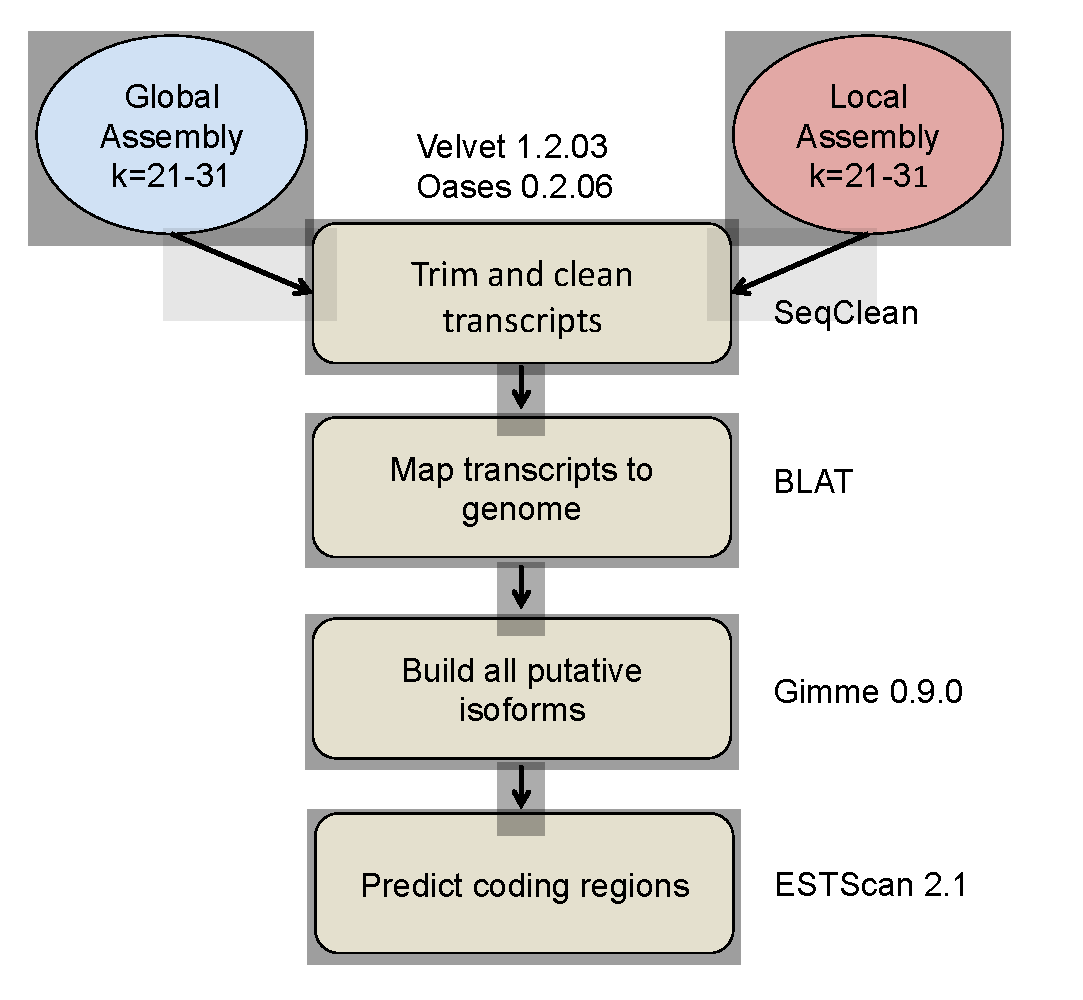
\includegraphics[width=5in]{overall_pipeline.pdf}
\end{center}
\caption{
{\bf Gene model construction pipeline.} Transcripts are obtained from two
assembly methods -- global and local assembly.  Transcripts are aligned to the
chicken genome by BLAT\@. Gimme then constructs gene models based on alignments
of transcripts.  }
\label{overall_pipeline}
\end{figure}

\begin{figure}[!ht]
\begin{center}
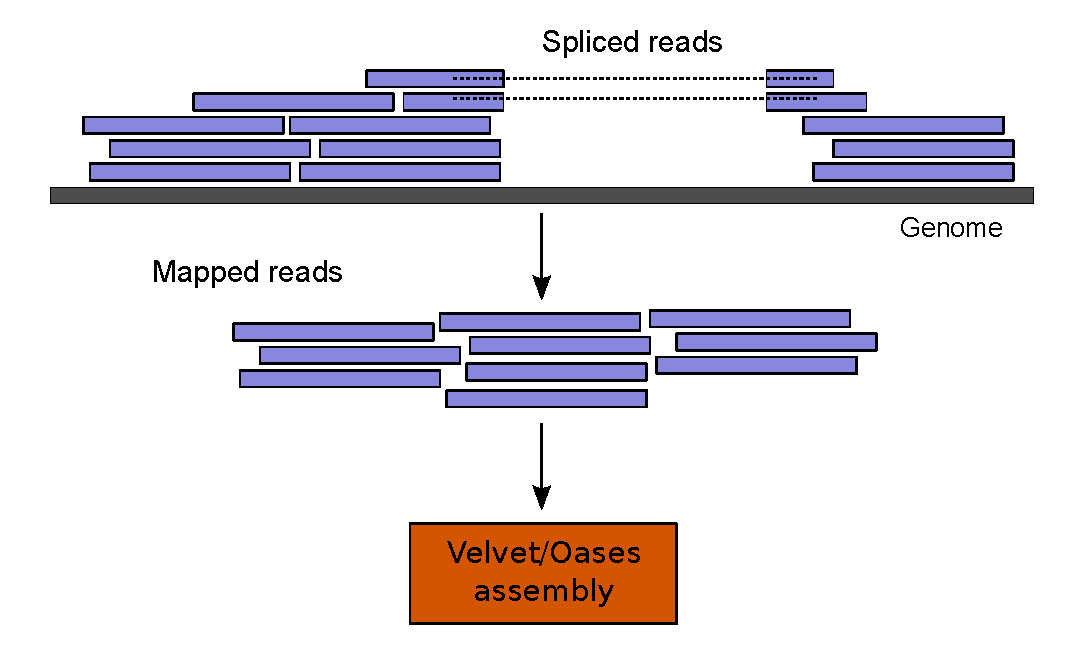
\includegraphics[width=5in]{local_assembly}
\end{center}
\caption{
{\bf Local Assembly Pipeline.}
Reads are first mapped to a chicken genome.  Then only mapped reads are
assembled by Velvet and Oases.
}
\label{local_assembly}
\end{figure}

\begin{figure}[!ht]
\begin{center}
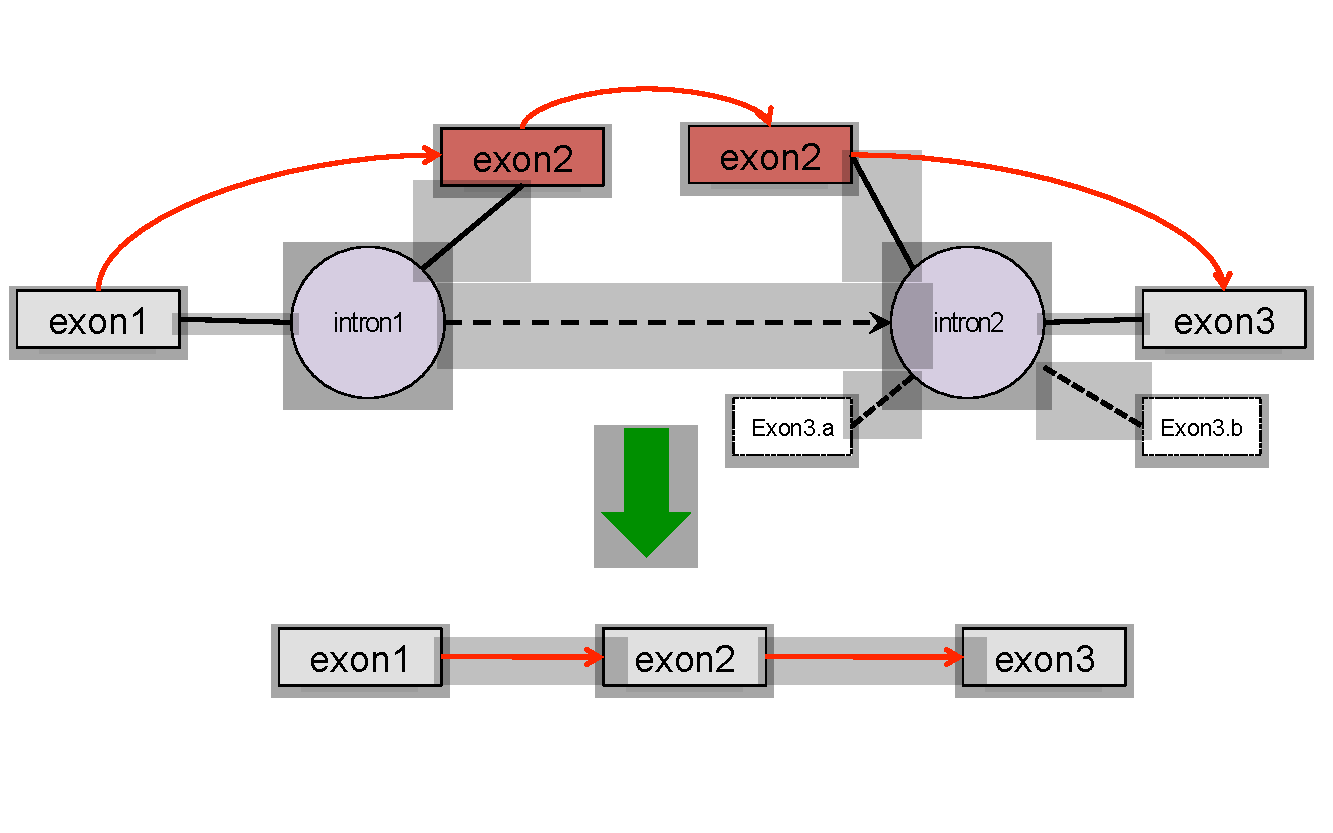
\includegraphics[width=5in]{algorithm.pdf}
\end{center}
\caption{
{\bf Intron and exon graphs.} Each intron connects to exons whose splice
junctions match it boundary.  Some exons are excluded from the final gene model
if they are incomplete (exon 3a,b).  Introns sharing at least one exon are
grouped together.  Then an exon graph is made using exons as nodes.
}
\label{algorithm}
\end{figure}

\begin{figure}[!ht]
\begin{center}
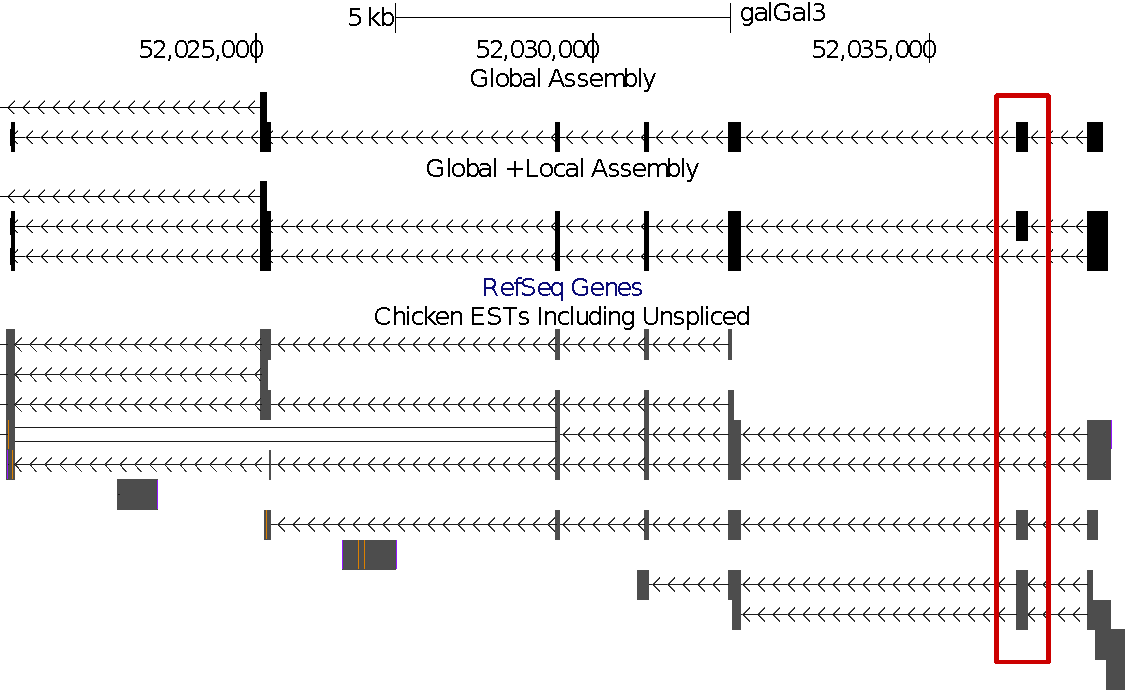
\includegraphics[width=5in]{global_vs_local.pdf}
\end{center}
\caption{
{\bf Global and local assembly detect different isoforms with the same k-mers.} 
}
\label{global_vs_local}
\end{figure}


% \begin{figure}[!ht]
% \begin{center}
% 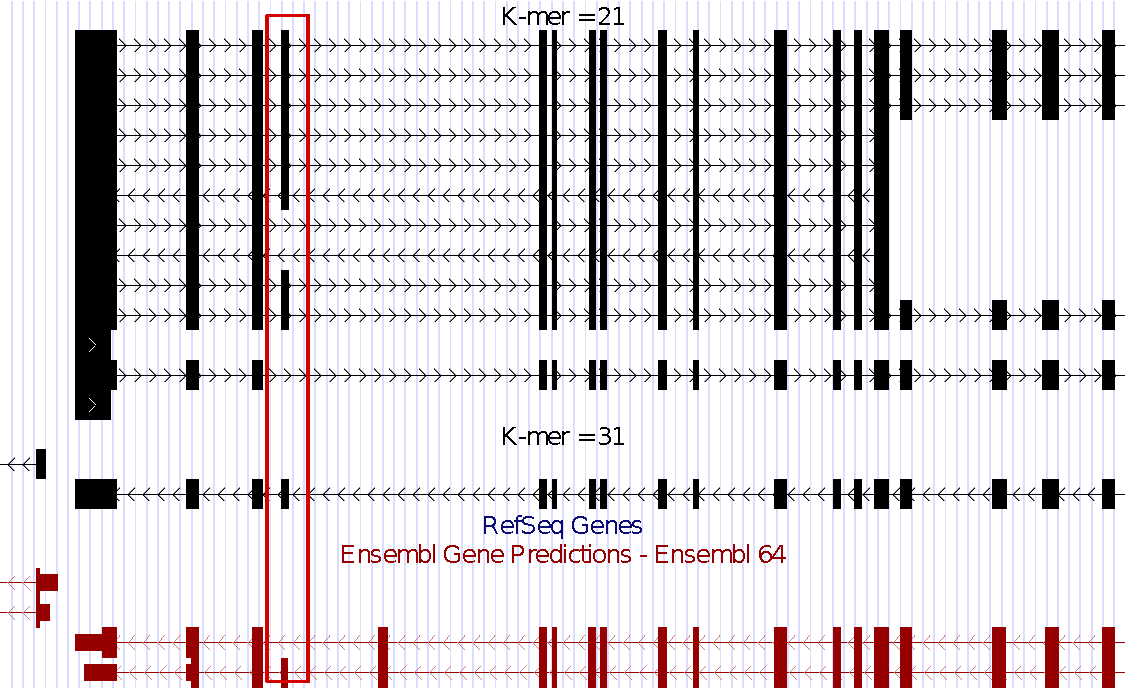
\includegraphics[width=5in]{kmers-variance.pdf}
% \end{center}
% \caption{
% {\bf Different isoforms are detected by different k-mer lengths.}
% K-mer=21 detects a skipped exon which is not detected by k-mer=31.
% The skipped exon is also annotated in Ensembl gene models.
% }
% \label{kmer-variance}
% \end{figure}

% \begin{figure}[!ht]
% \begin{center}
% 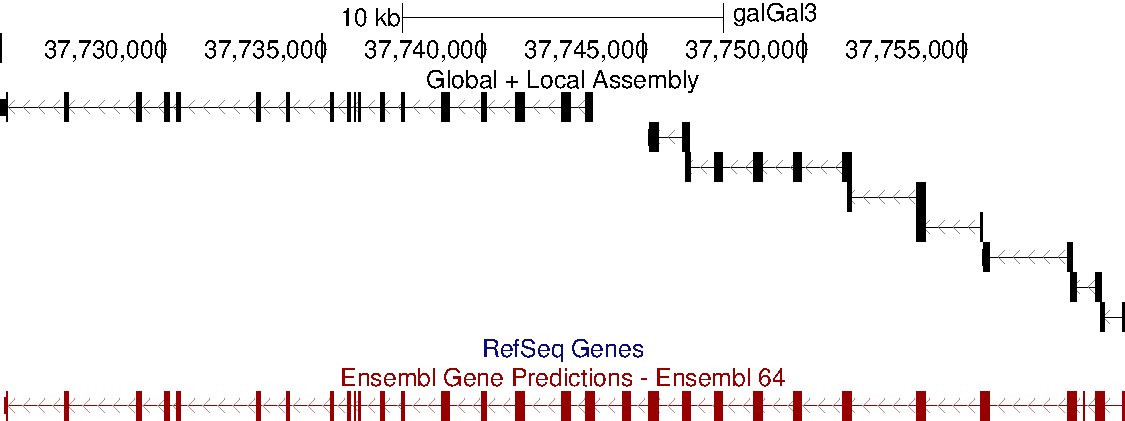
\includegraphics[width=5in]{fragmented_transcripts.pdf}
% \end{center}
% \caption{
% {\bf Example of fragmented transcripts near $5'$ end of a long transcript.}
% }
% \label{fragmented_transcripts}
% \end{figure}

% \begin{figure}[!ht]
% \begin{center}
% 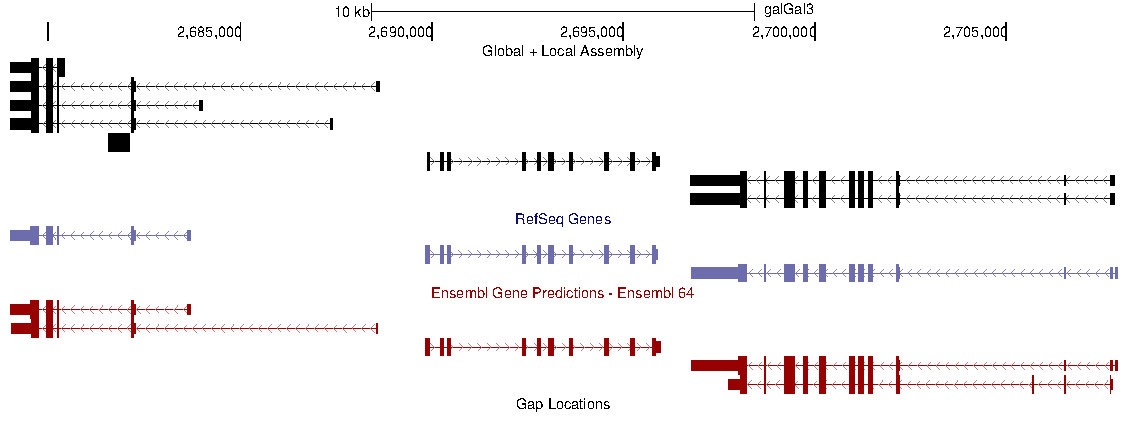
\includegraphics[width=5in]{model_comparisons.pdf}
% \end{center}
% \caption{
% {\bf Comparison of gene models from the \emph{de novo} assembly pipeline with
% reference and Ensembl gene models on UCSC genome browser.}
% }
% \label{model_comparisons}
% \end{figure}

% \begin{figure}[!ht]
% \begin{center}
% 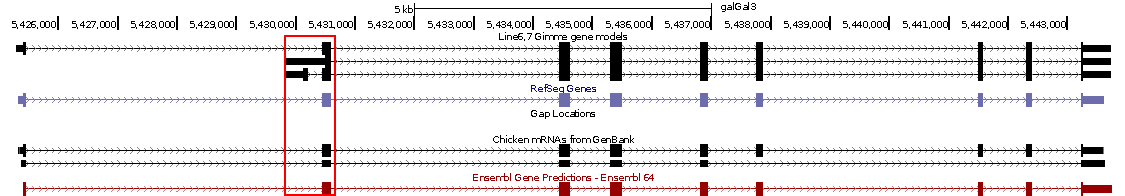
\includegraphics[width=6in]{alter_5utr.pdf}
% \end{center}
% \caption{
% {\bf Examples of alternative $5'$ UTRs in RNA-Seq gene models.}
% }
% \label{alter_5utr}
% \end{figure}
% 
% \begin{figure}[!ht]
% \begin{center}
% 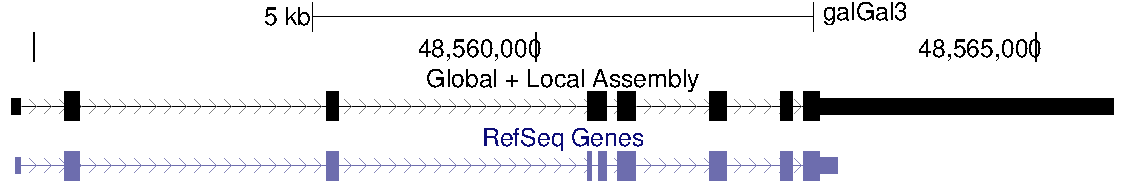
\includegraphics[width=5in]{long_utr.pdf}
% \end{center}
% \caption{
% {\bf Examples of an extended $3'$ UTR in RNA-Seq gene models.}
% }
% \label{long_utr}
% \end{figure}

\begin{figure}[!ht]
\begin{center}
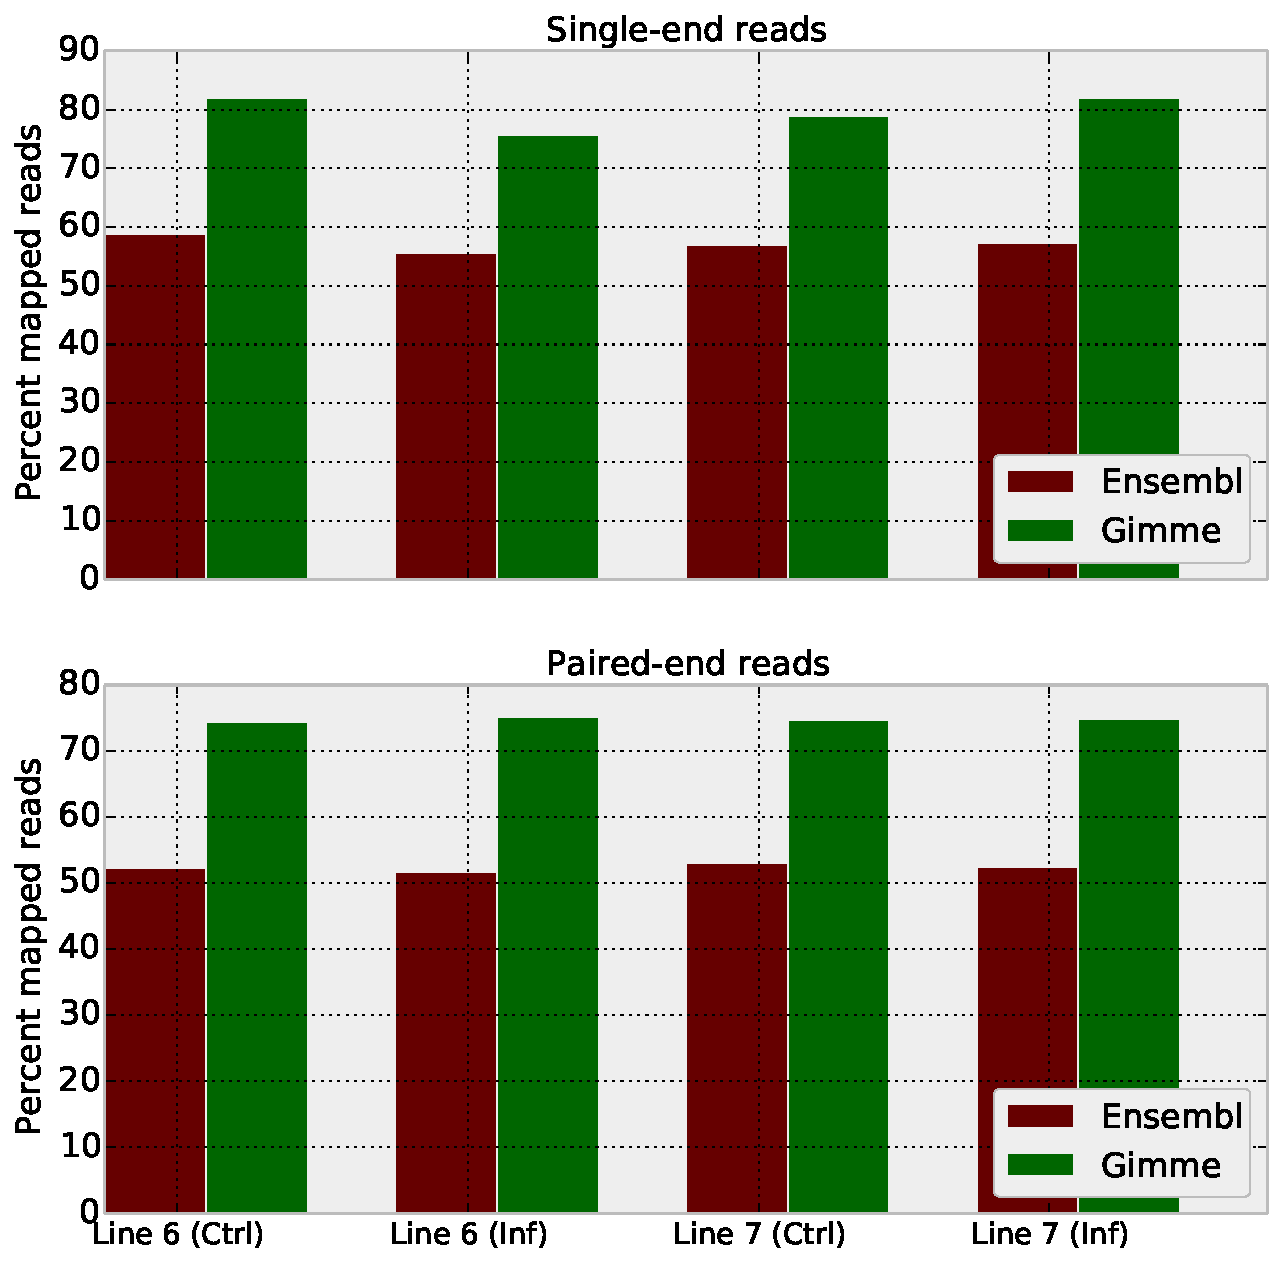
\includegraphics[width=5in]{mapped-reads.pdf}
\end{center}
\caption{
{\bf Cumulative counts of splice junctions with spliced reads from both single-
and paired-end data from Cufflinks and Gimme models.}
}
\label{mapped-reads}
\end{figure}

\begin{figure}[!ht]
\begin{center}
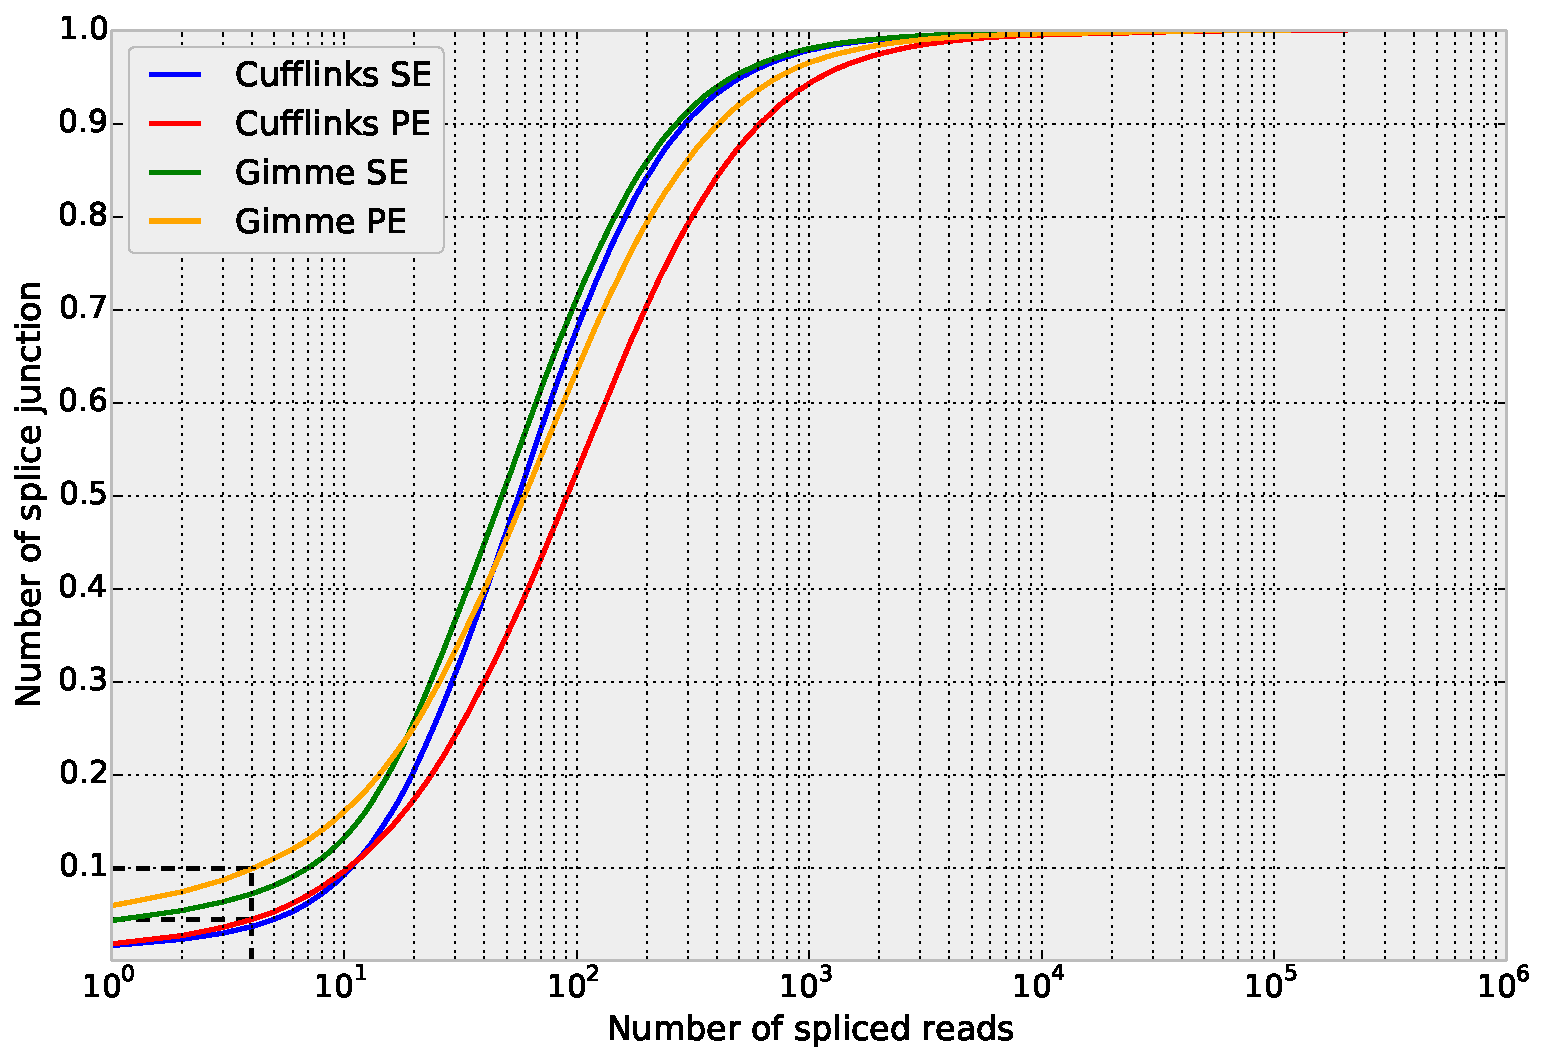
\includegraphics[width=5in]{cdf_splice.pdf}
\end{center}
\caption{
{\bf Cumulative counts of splice junctions with spliced reads from single- and
paired-end data.}
}
\label{cdf_splice}
\end{figure}

\begin{figure}[!ht]
\begin{center}
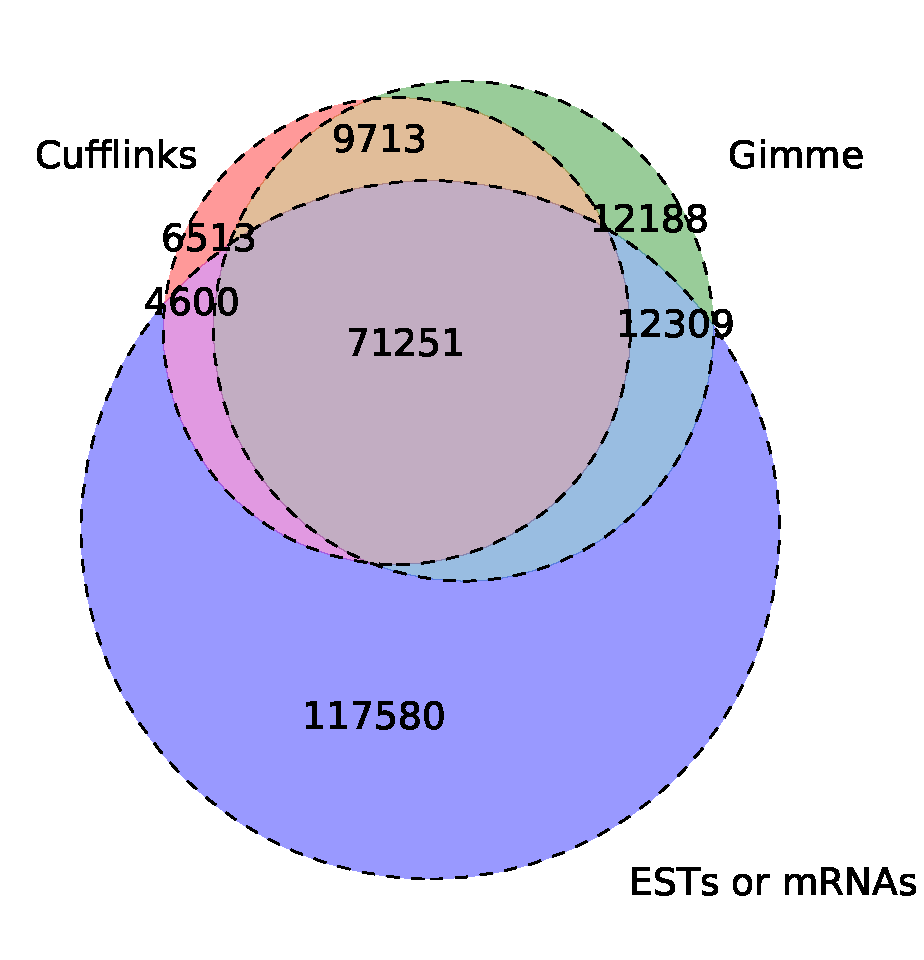
\includegraphics[width=5in]{chick_est_venn.pdf}
\end{center}
\caption{
    {\bf Splice junctions supported by ESTs or mRNAs.}
}
\label{chick_est_venn}
\end{figure}

\begin{figure}[!ht]
\begin{center}
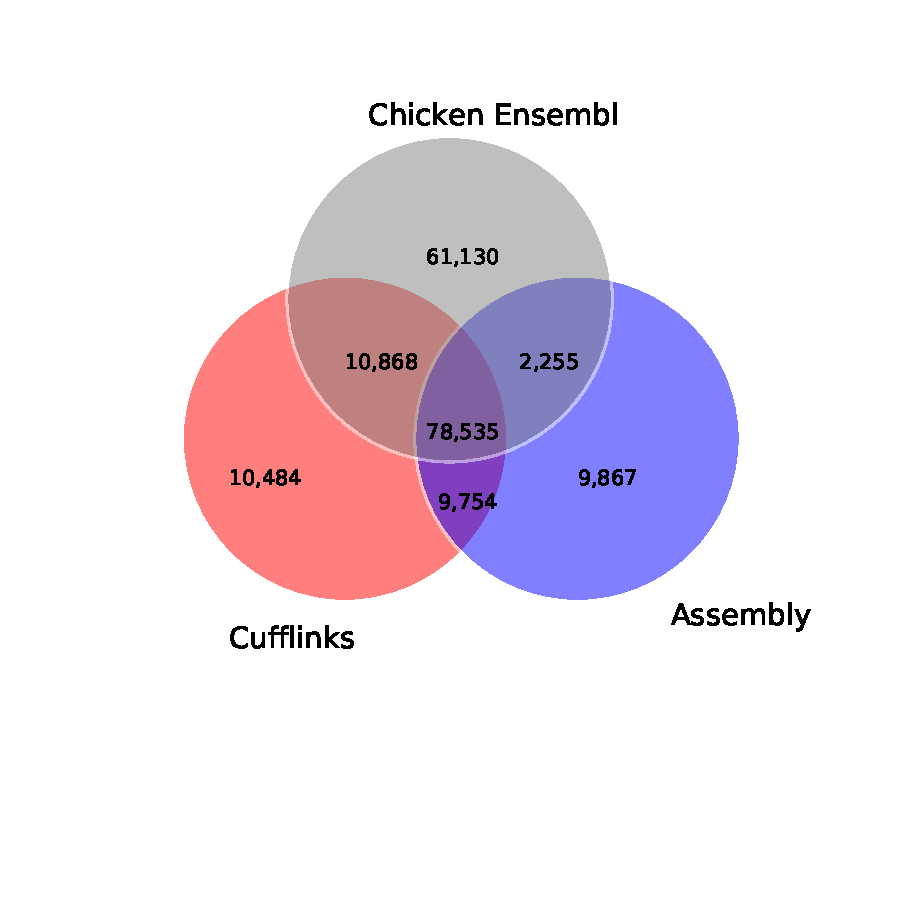
\includegraphics[width=5in]{chick_venn.pdf}
\end{center}
\caption{
{\bf Splice sites in chicken Ensembl gene models detected by Cufflinks and the
{\em de novo} assembly pipeline.} Cufflinks detects many annotated isoforms
that are not detected by the pipeline.  The figure also shows that both methods
detect a large number of unannotated splice junctions.}
\label{chick_venn}
\end{figure}


\begin{figure}[!ht]
\begin{center}
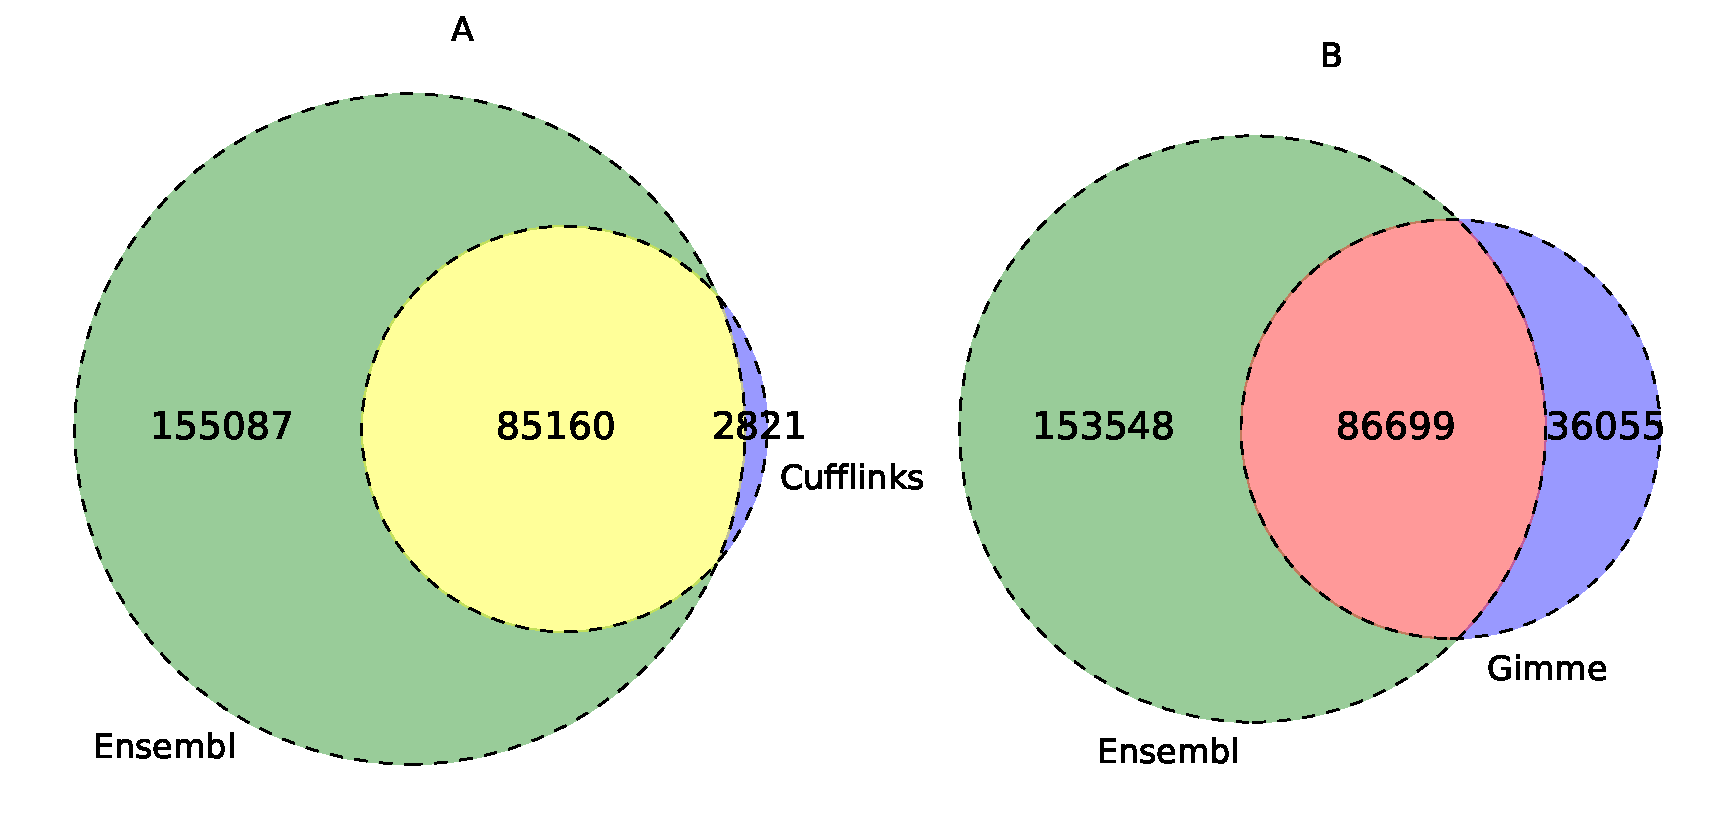
\includegraphics[width=5in]{mouse_venn.pdf}
\end{center}
\caption{
{\bf Splice sites in mouse Ensembl gene models, Cufflinks and the \emph{de
novo} assembly pipeline.} In contrast to chicken datasets, 85,160 (96.8\%) of
splice junctions found by Cufflinks are annotated in mouse ENSEMBL models. The
higher percentage of ENSEMBL splice junctions found by Cufflinks may be a
result of more complete ENSEMBL gene models. While Gimme can detect the similar
number of ENSEMBL splice junctions, it detects many more non-ENSEMBL splice
junctions in mouse.}
\label{mus_venn}
\end{figure}


\begin{figure}[!ht]
\begin{center}
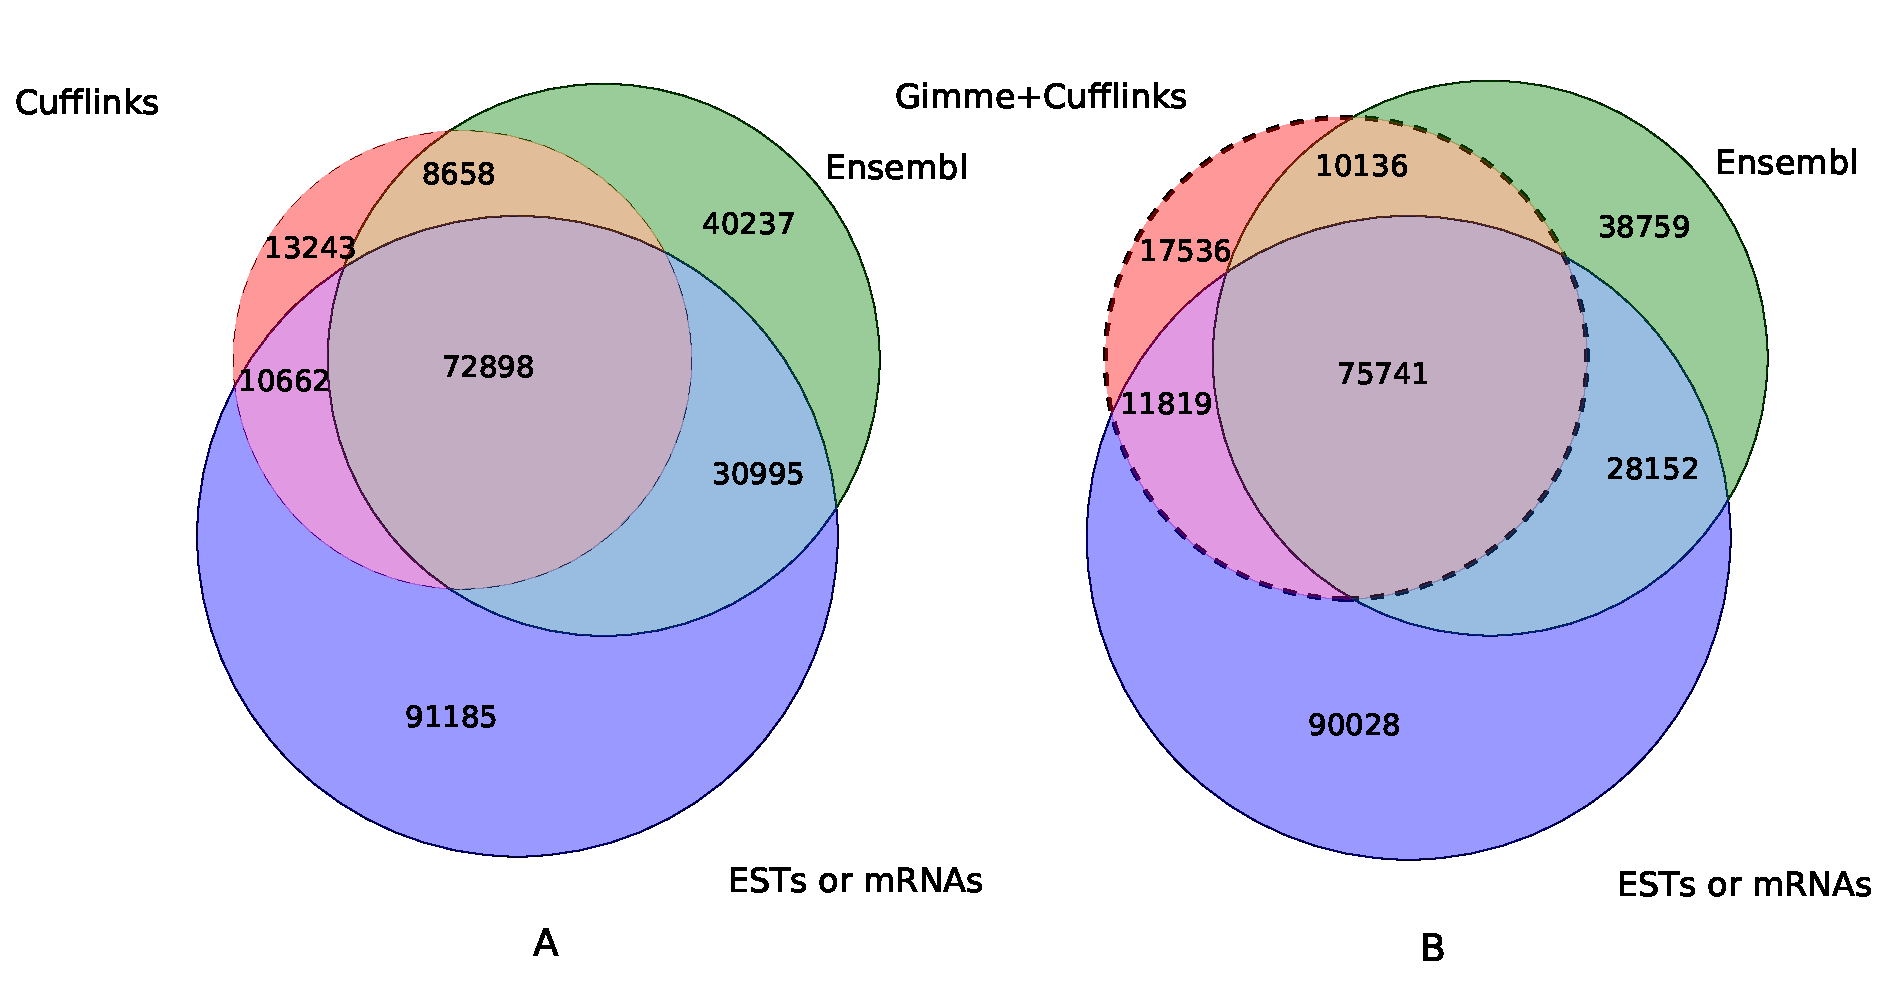
\includegraphics[width=5in]{cuff_gimme_junctions_venn.pdf}
\end{center}
\caption{
    {\bf Splice junctions found in merged models.} Merged models (B) find more
    splice junctions in ENSEMBL and ESTs + mRNAs than Cufflinks models only (A).
}
\label{combined_venn}
\end{figure}

% \begin{figure}[!ht]
% \begin{center}
% \includegraphics[width=5in]{chick_est_mrna_venn.pdf}
% \end{center}
% \caption{
% {\bf Splice sites in Chicken ESTs and mRNAs not included in Ensembl detected by
% Cufflinks and the \emph{de novo} assembly pipeline.}
% Both Cufflinks and our pipeline find splice junctions not included in Ensembl
% but supported by EST and mRNA sequences.
% }
% \label{chick_est_mrna_venn}
% \end{figure}

\begin{figure}[!ht]
\begin{center}
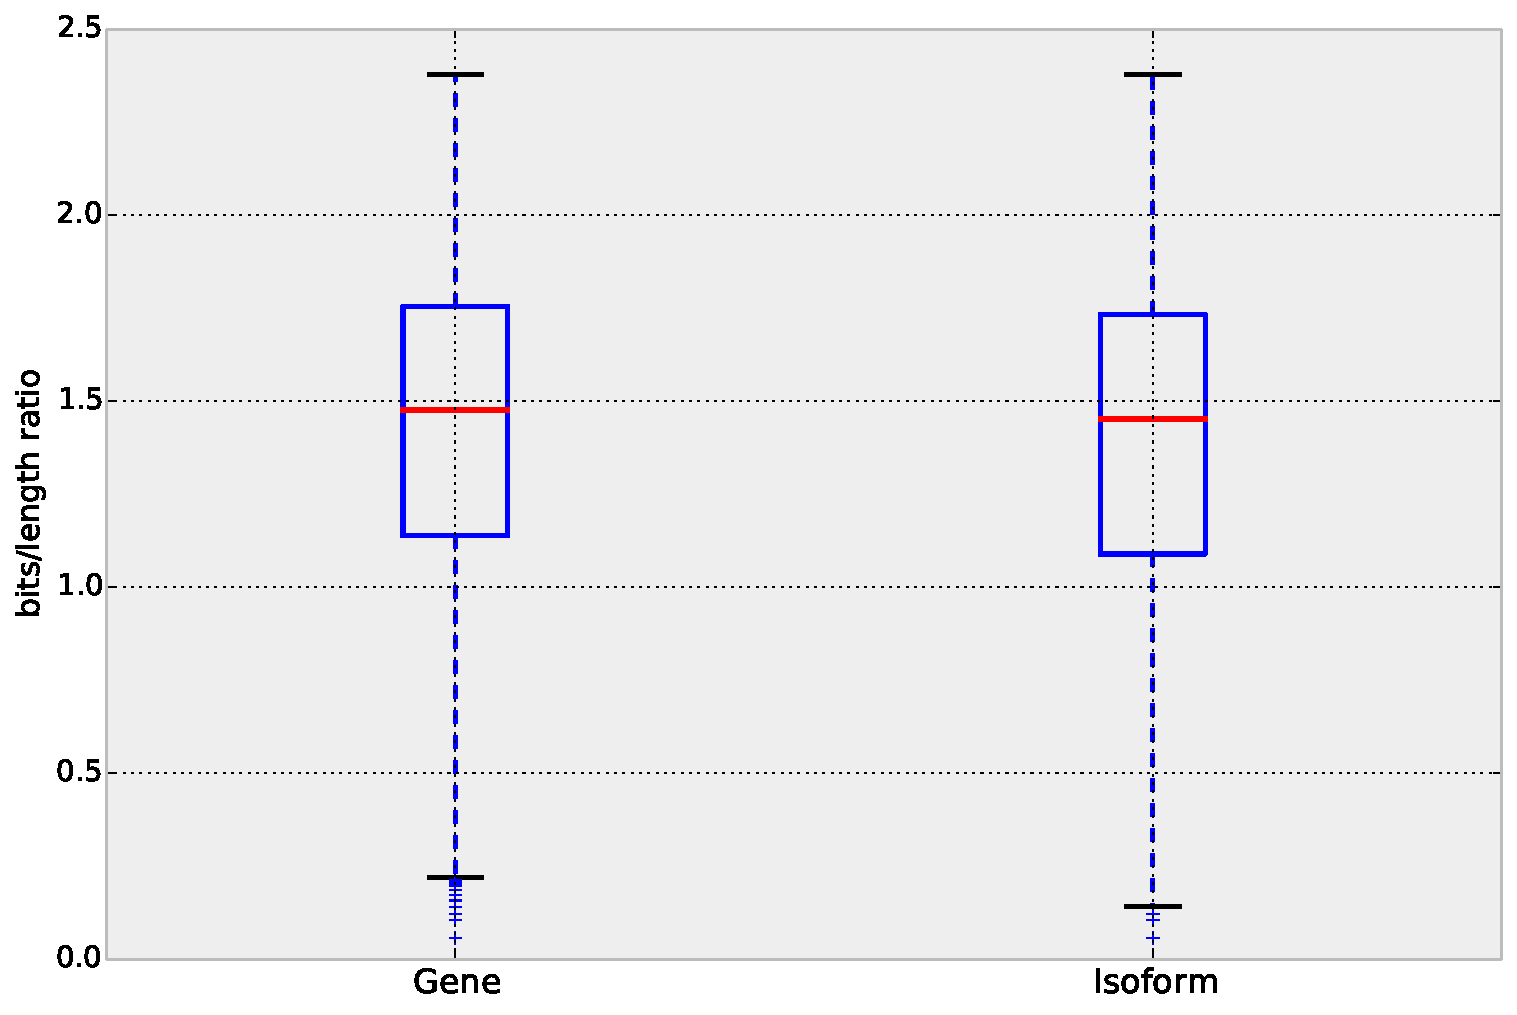
\includegraphics[width=5in]{mouse-homolog-boxplot.pdf}
\end{center}
\caption{
{\bf Box plots of bit score/length ratio of isoforms and genes that match mouse
proteins.} Only the greatest ratio of isoforms from the same gene is plotted for
the gene plot. Ratios from every isoform are plotted for the isoform plot.}
\label{bitscore}
\end{figure}

% \begin{figure}[!ht]
% \begin{center}
% 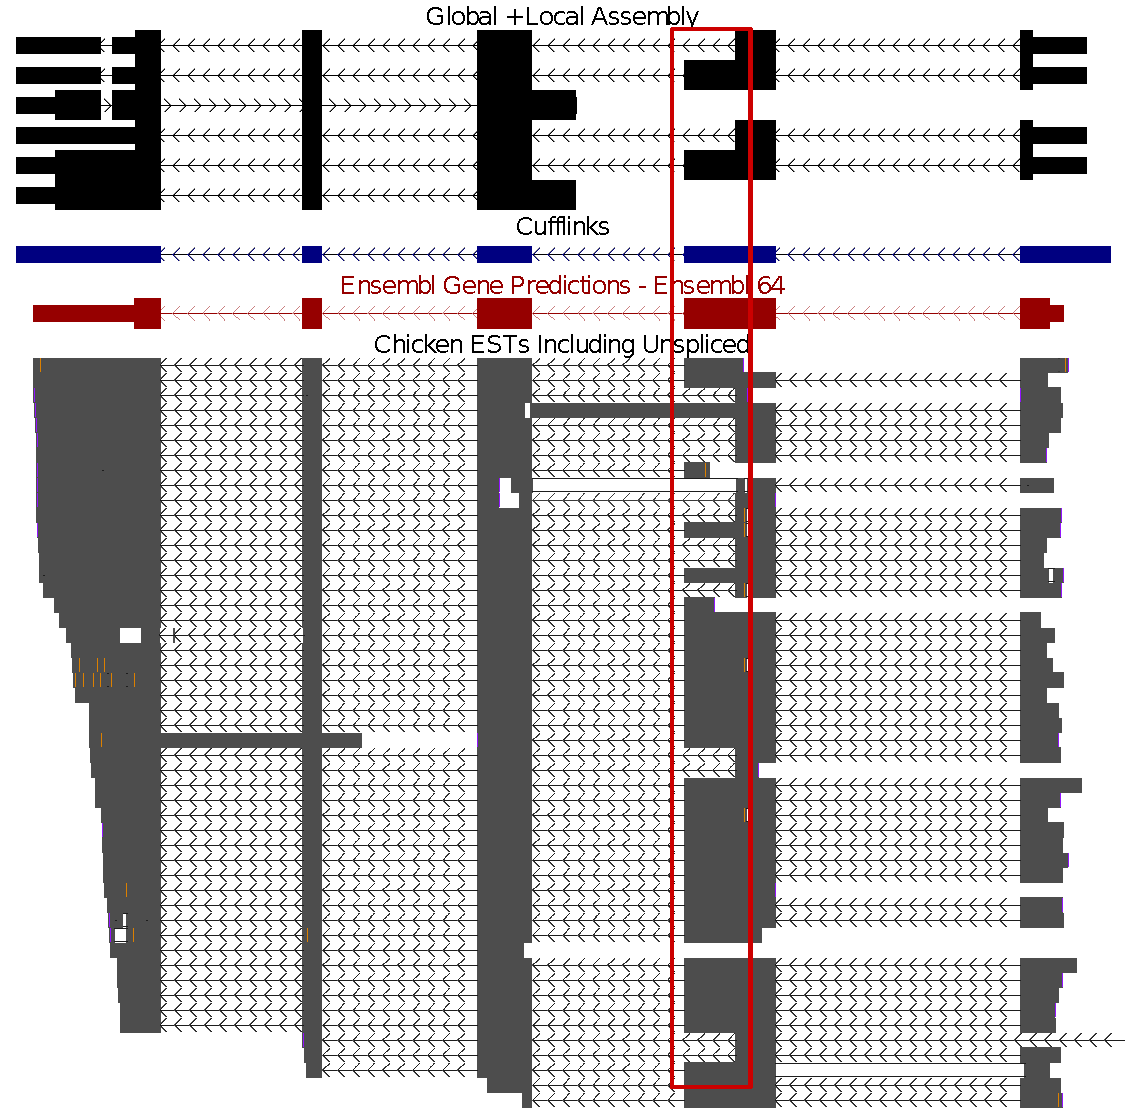
\includegraphics[width=5in]{alt_splice_site.pdf}
% \end{center}
% \caption{
% {\bf Unannotated alternative splice site.} The pipeline detects alternative
% splices site not annotated in Ensembl and Cufflinks but are supported by ESTs.
% }
% \label{alt_splice_site}
% \end{figure}
% 
% \begin{figure}[!ht]
% \begin{center}
% 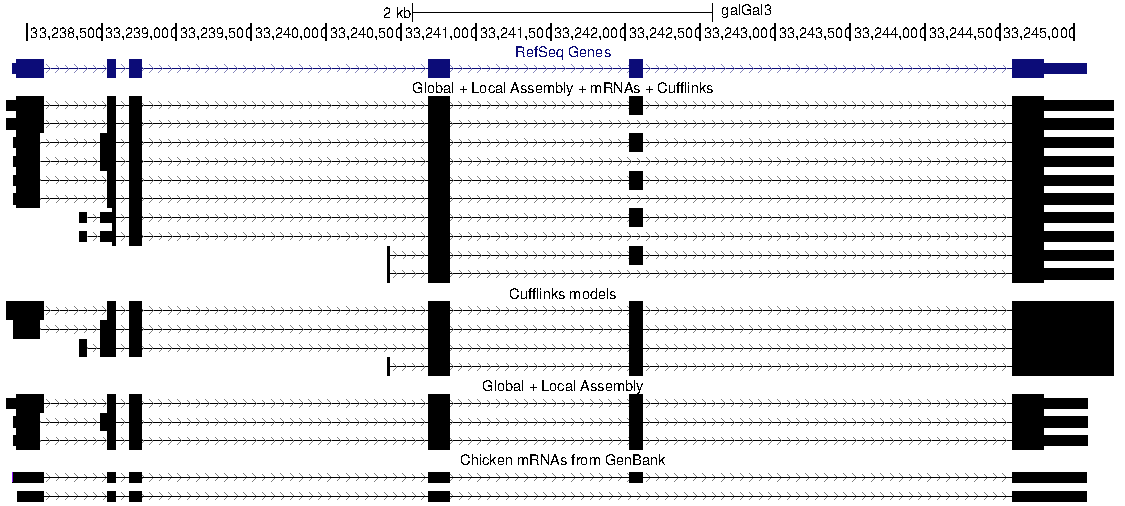
\includegraphics[width=5in]{mrna_cuff_gimme.pdf}
% \end{center}
% \caption{
% {\bf mRNAs + Cufflinks + Assembly gene models.} Gimme can combine transcripts
% from different sources to build gene models.  In this figure, the final gene
% model includes several isoforms not annotated in the reference gene model.  }
% \label{mrna_cuff_gimme}
% \end{figure}

\end{document}
